
% prime_en.tex — Edges of Counting and Computation — Prime — Revised for deposit
% Compiler: XeLaTeX or pdfLaTeX
\documentclass[12pt,a4paper]{article}
\usepackage{amsmath,amssymb}
\usepackage{graphicx}
\usepackage{booktabs}
\usepackage{array}
\usepackage[margin=2.2cm]{geometry}
\usepackage{xcolor}
\usepackage{float}
\usepackage{hyperref}
\usepackage{fancyhdr}
\pagestyle{fancy}
\fancyhf{}
\fancyhead[L]{\small Edges of Counting and Computation — Prime}
\fancyhead[R]{\small M. N. Al-Jabri (2026)}
\fancyfoot[L]{\scriptsize Abdulla M. N. Al-Jabri | ORCID: 0009-0003-3319-3822}
\fancyfoot[C]{\scriptsize Zenodo DOI: to be assigned}
\fancyfoot[R]{\small \thepage}
\renewcommand{\headrulewidth}{0.4pt}
\renewcommand{\footrulewidth}{0.4pt}
\fancypagestyle{firstpage}{
  \fancyhf{}
  \fancyfoot[C]{\small Abdulla M. N. Al-Jabri — Edges of Counting and Computation — Prime — \thepage}
  \renewcommand{\headrulewidth}{0pt}
  \renewcommand{\footrulewidth}{0pt}
}
\title{\textbf{Edges of Counting and Computation — Prime}\\
\large Cross-Stage Empirical Synthesis ($A \rightarrow D$) up to $10^9$}
\author{Abdulla Mohammed Nasser Al-Jabri \\
Sana'a, Republic of Yemen \\
ORCID: 0009-0003-3319-3822 \\
Email: \texttt{jabri62018@gmail.com} \\
Portal: \url{https://jabri-com.vercel.app} \\
Zenodo DOI: to be assigned on deposit}
\date{November 21, 2026}
\begin{document}
\maketitle
\thispagestyle{firstpage}

% --- Reproducibility — first page, DOI/Zenodo ---
\begin{center}
\fbox{\parbox{0.92\textwidth}{
\textbf{Reproducibility and Computational Materials}\\[2mm]
The computational scripts, data-processing procedures, and supporting materials used to generate the reported results are available at:\\[1mm]
\textbf{GitHub Repository:} [Repository Link]\\[1mm]
\textbf{Archived Release:} [Release Link]\\[1mm]
The archived release corresponds to the version used in this study and provides the materials needed to inspect and reproduce the reported computations. Reproducibility materials cover only the results already presented in this paper; no reproduction is promised for tests not yet closed, including M1-E, until they are closed and their version is fixed.
}}
\end{center}
\vspace{0.3cm}

\begin{center}
\textbf{We count primes, compute their edges (gaps), and present what comparisons across ranges showed.}
\end{center}
% ==========================================
\begin{abstract}
This study presents the results of a computational survey and analysis of prime gaps within a specified range, documenting the method of data extraction, measurements, and tests used. Evaluation of the results, their implications, and the place of this work is left to the reader and referees.

The paper investigates the statistical behaviour of consecutive prime gaps $g_n = p_{n+1} - p_n$ up to $N = 10^9$. We track the prime counting function $\pi(x)$, logarithmic integral deviations $D_1(x) = \pi(x) - \mathrm{Li}(x)$ and $D_2(x) = \pi(x) - x/\ln x$, local window densities $\rho_k$, and gap frequency rankings across four comparative ranges ($A, B, C, D$), which are segments of the same computational sequence, not statistically independent runs.

At the documented closure checkpoints, $D_1(x)$ was negative ($-1,699.912$ at $10^9$). Local density decreased across the nine measured windows of Stage $D$ ($0.053175 \rightarrow 0.048383$), consistent with the prime number theorem. Gap frequency ranking differed across the compared ranges: in Stage $D$, gap $10$ ranked above gaps $4$ and $2$. The lag-1 correlation on the class sequence was $r_1 = -0.03006$ in $M1$, on the encoding documented below. The study explores the relation between changing prime density and gap distribution, without assuming a prior causal relation.
\end{abstract}
% ==========================================
\section{Introduction, Problem Statement, and Hypothesis}
While prime numbers are deterministically defined, their local spacing exhibits intricate statistical behavior that raises questions regarding short-range association and modular constraints.
\begin{itemize}
    \item \textbf{Research Question:} Do consecutive prime gaps carry statistical ``memory'' or invariant structural patterns across increasing numerical scales? Here ``memory'' is used in an operational statistical sense, i.e.\ a measurable association between one gap and a later gap, not a mechanism inside the prime numbers.
    \item \textbf{Pre-Computation Null Hypothesis:} We initially hypothesised that gap sizes behave as statistically independent variables and that the relative frequency ranking of the most common gaps ($2, 4, 6, 10, 12, \dots$) remains stable across ranges $A, B, C,$ and $D$.
    \item \textbf{Methodological Rule:} Every observation is recorded if backed by a verified number in its respective range.
\end{itemize}
\noindent \textbf{What this work presents:} extraction of the gap sequence up to one billion, measurement of deviation from $\mathrm{Li}(x)$, tracking of changing prime density, analysis of gap-size distribution, comparison of gap frequency rankings across ranges, testing of correlation between consecutive gaps, and a sharper test of whether the exact gap value adds information beyond its class.
% ==========================================
\section{Official Research Identity}
\begin{figure}[H]
\centering
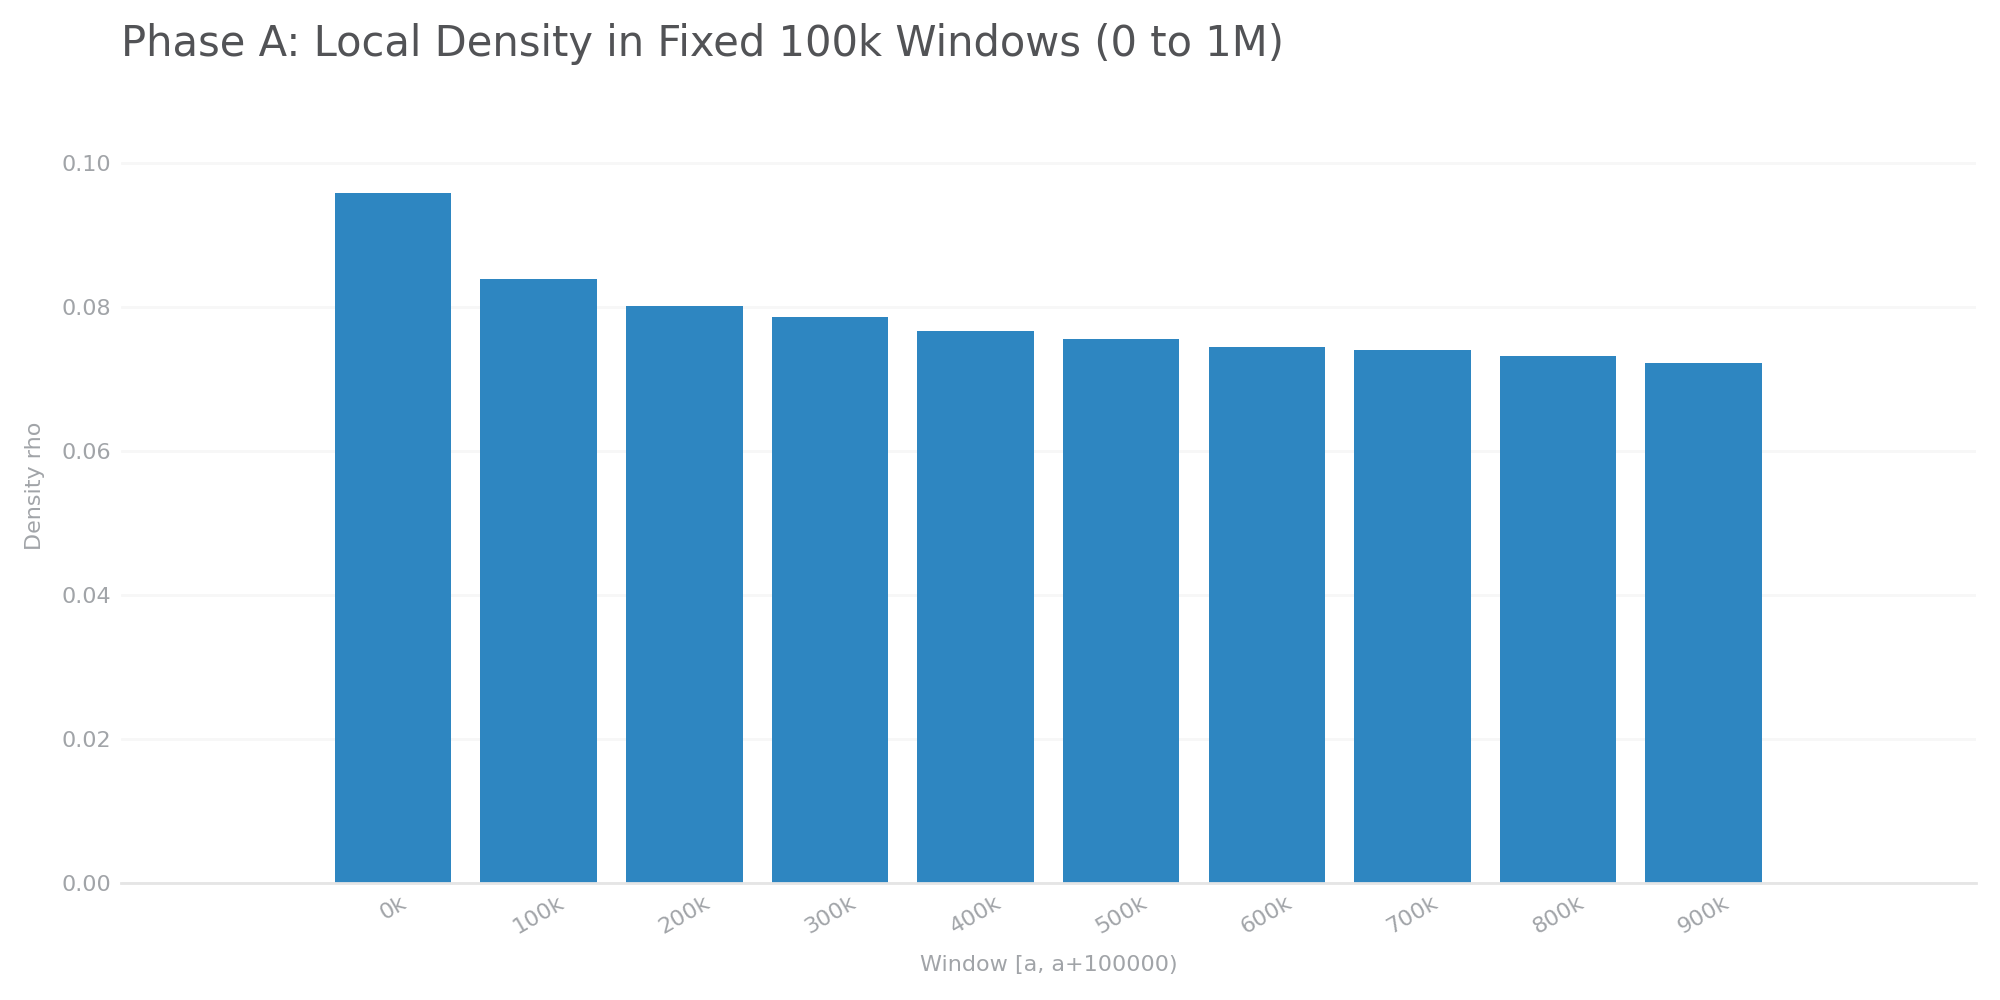
\includegraphics[width=0.90\textwidth]{prime1.png}
\caption{Official Research Identity Card — Prime}
\end{figure}
\begin{table}[H]
\centering
\begin{tabular}{ll}
\toprule
\textbf{Attribute} & \textbf{Value} \\
\midrule
Author & Abdulla Mohammed Nasser Al-Jabri \\
Affiliation / Location & Sana'a, Republic of Yemen \\
ORCID & 0009-0003-3319-3822 \\
Email & \texttt{jabri62018@gmail.com} \\
Research Portal & \url{https://jabri-com.vercel.app} \\
Work Title & Edges of Counting and Computation — Prime \\
Mathematical Definition & $g_n = p_{n+1} - p_n$ \\
Computational Horizon & $N = 10^9$ ($\pi(10^9) = 50,847,534$) \\
Zenodo DOI & to be assigned on deposit \\
Date & November 21, 2026 \\
\bottomrule
\end{tabular}
\caption{Research Metadata and Reference Parameters}
\end{table}
% ==========================================
\section{Definitions and Mathematical Protocol}
\subsection{The Edge (Prime Gap)}
An edge $g_n$ is defined as the arithmetic difference between two consecutive primes:
\[
g_n = p_{n+1} - p_n, \quad \forall n \geq 1
\]
\begin{enumerate}
    \item \textbf{Sieve Protocol:} Primes are generated via the Sieve of Eratosthenes up to $N$, with $1$ explicitly excluded from the prime set.
    \item \textbf{Unique Odd Edge:} The initial edge $g_1 = 3 - 2 = 1$ is the sole odd gap in the sequence. Every prime $p_n > 2$ is odd, making every subsequent gap strictly even ($g_n \equiv 0 \pmod 2$ for all $n \geq 2$).
\end{enumerate}
\subsection{Counting, Deviation, and Density Functions}
\begin{itemize}
    \item $\pi(x)$: Exact count of primes $\leq x$.
    \item $\mathrm{Li}(x) = \mathrm{Ei}(\ln x) - \mathrm{Ei}(\ln 2) = \int_2^x \frac{dt}{\ln t}$: Offset logarithmic integral.
    \item $D_1(x) = \pi(x) - \mathrm{Li}(x)$ and $D_2(x) = \pi(x) - x/\ln x$.
    \item $R(x) = |D_1(x)| / \pi(x)$: Relative logarithmic deviation.
    \item $\rho_k = (\pi(b_k) - \pi(a_k)) / 10^8$: Local prime density in window $k$. $\bar{g}_k = 1/\rho_k$ is the Estimated Mean Spacing in window $k$, derived from density; it is not the directly computed mean of the gaps in that window, which would be $\bar{g}_k^{\,\mathrm{actual}} = (1/m_k)\sum_{j=1}^{m_k} g_j$. The two values may differ slightly because of window boundaries and endpoint inclusion.
\end{itemize}
\subsection{Stage $D$ Inclusion Rule and $M1$ Size Classes}
A gap $g_n = p_{n+1} - p_n$ is counted inside Stage $D$ if and only if its upper endpoint satisfies $p_{n+1} > 10^8$ ($100\text{M}$), yielding exactly $45,086,079$ gaps in Stage $D$. Gaps are partitioned into three exhaustive $M1$ classes:
\begin{itemize}
    \item \textbf{Small:} $g \leq 6$ ($\{1, 2, 4, 6\}$).
    \item \textbf{Medium:} $8 \leq g \leq 14$ ($\{8, 10, 12, 14\}$).
    \item \textbf{Large:} $g \geq 16$.
\end{itemize}
Because $g_1 = 1$ falls inside the Small class and all subsequent gaps are even, no odd integers ($7$ or $15$) exist between class boundaries.
% ==========================================
\section{Cross-Stage Synthesis ($A \rightarrow D$) and Results}
\subsection{Closure Comparison Across Stages $A$--$D$}
\begin{table}[H]
\centering\small
\begin{tabular}{llrrrrr}
\toprule
\textbf{Stage} & \textbf{Range} & \textbf{Window} & $\pi(x)$ & $D_1 = \pi - \mathrm{Li}$ & $D_2 = \pi - x/\ln x$ & $R = |D_1|/\pi$ \\
\midrule
$A$ & Up to $10^6$ & $10^5$ & $78,498$ & $-128.504$ & $+6,115.586$ & $0.001637035$ \\
$B$ & Up to $10^7$ & $10^6$ & $664,579$ & $-338.360$ & $+44,158.312$ & $0.000509134$ \\
$C$ & Up to $10^8$ & $10^7$ & $5,761,455$ & $-753.330$ & $+332,773.976$ & $0.000130753$ \\
$D$ & $10^8 \rightarrow 10^9$ & $10^8$ & $50,847,534$ & $-1,699.912$ & $+2,592,591.566$ & $0.000033432$ \\
\bottomrule
\end{tabular}
\caption{Closure comparison across Stages $A, B, C,$ and $D$. Values are documented checkpoints.}
\end{table}
\subsection{Stage $D$ Cumulative Checkpoints (Every $100\text{M}$)}
\begin{table}[H]
\centering\small
\begin{tabular}{rrrrrrr}
\toprule
$x$ & $\pi(x)$ & $\mathrm{Li}(x)$ & $D_1$ & $\Delta D_1$ & $D_2$ & $R(x)$ \\
\midrule
$100{,}000{,}000$ & $5{,}761{,}455$ & $5{,}762{,}208.3$ & $-753.3$ & $-753.3$ & $332{,}774.0$ & $0.000131$ \\
$200{,}000{,}000$ & $11{,}078{,}937$ & $11{,}079{,}973.8$ & $-1{,}036.8$ & $-283.5$ & $615{,}308.2$ & $0.000094$ \\
$300{,}000{,}000$ & $16{,}252{,}325$ & $16{,}253{,}408.1$ & $-1{,}083.1$ & $-46.3$ & $882{,}915.9$ & $0.000067$ \\
$400{,}000{,}000$ & $21{,}336{,}326$ & $21{,}337{,}377.0$ & $-1{,}051.0$ & $+32.1$ & $1{,}141{,}420.0$ & $0.000049$ \\
$500{,}000{,}000$ & $26{,}355{,}867$ & $26{,}356{,}831.1$ & $-964.1$ & $+86.9$ & $1{,}393{,}458.7$ & $0.000037$ \\
$600{,}000{,}000$ & $31{,}324{,}703$ & $31{,}326{,}044.207$ & $-1{,}341.207$ & $-377.103$ & $1{,}640{,}014.082$ & $0.000042816$ \\
$700{,}000{,}000$ & $36{,}252{,}931$ & $36{,}254{,}240.999$ & $-1{,}309.999$ & $+31.208$ & $1{,}882{,}917.694$ & $0.000036135$ \\
$800{,}000{,}000$ & $41{,}146{,}179$ & $41{,}147{,}861.2$ & $-1{,}682.2$ & $-372.2$ & $2{,}122{,}021.5$ & $0.000041$ \\
$900{,}000{,}000$ & $46{,}009{,}215$ & $46{,}011{,}647.6$ & $-2{,}432.6$ & $-750.4$ & $2{,}357{,}836.0$ & $0.000053$ \\
$1{,}000{,}000{,}000$ & $50{,}847{,}534$ & $50{,}849{,}233.912$ & $-1{,}699.912$ & $+732.688$ & $2{,}592{,}591.566$ & $0.000033432$ \\
\bottomrule
\end{tabular}
\caption{Cumulative checkpoints across Stage $D$. Negativity of $D_1$ is observed at these checkpoints.}
\end{table}
\subsection{Window Density and Top 15 Gap Frequencies in Stage $D$}
Across the nine $100\text{M}$ windows of Stage $D$, local prime density $\rho_k$ decreased from $0.053175$ ($100\text{M}$--$200\text{M}$) to $0.048383$ ($900\text{M}$--$1\text{B}$), while the mean gap $\bar{g}_k$ rose from $18.806$ to $20.668$. The maximum observed gap inside Stage $D$ was $g = 282$ between $436{,}273{,}009$ and $436{,}273{,}291$.
\begin{table}[H]
\centering
\begin{tabular}{rrr}
\toprule
\textbf{Rank} & \textbf{Gap} & \textbf{Count in $D$} \\
\midrule
1 & 6 & $5{,}321{,}039$ \\
2 & 12 & $3{,}930{,}575$ \\
3 & 10 & $3{,}054{,}751$ \\
4 & 4 & $2{,}984{,}422$ \\
5 & 2 & $2{,}984{,}194$ \\
6 & 18 & $2{,}966{,}294$ \\
7 & 8 & $2{,}360{,}929$ \\
8 & 14 & $2{,}171{,}364$ \\
9 & 24 & $2{,}109{,}926$ \\
10 & 30 & $1{,}955{,}144$ \\
11 & 16 & $1{,}630{,}293$ \\
12 & 20 & $1{,}621{,}121$ \\
13 & 22 & $1{,}393{,}734$ \\
14 & 28 & $1{,}089{,}676$ \\
15 & 36 & $1{,}057{,}496$ \\
\bottomrule
\end{tabular}
\caption{Top 15 prime gap frequencies in Stage $D$ — Total in $D$: $45,086,079$}
\end{table}
\subsection{Visual Diagnostics ($B$, $C$, and $D$)}
\begin{figure}[H]\centering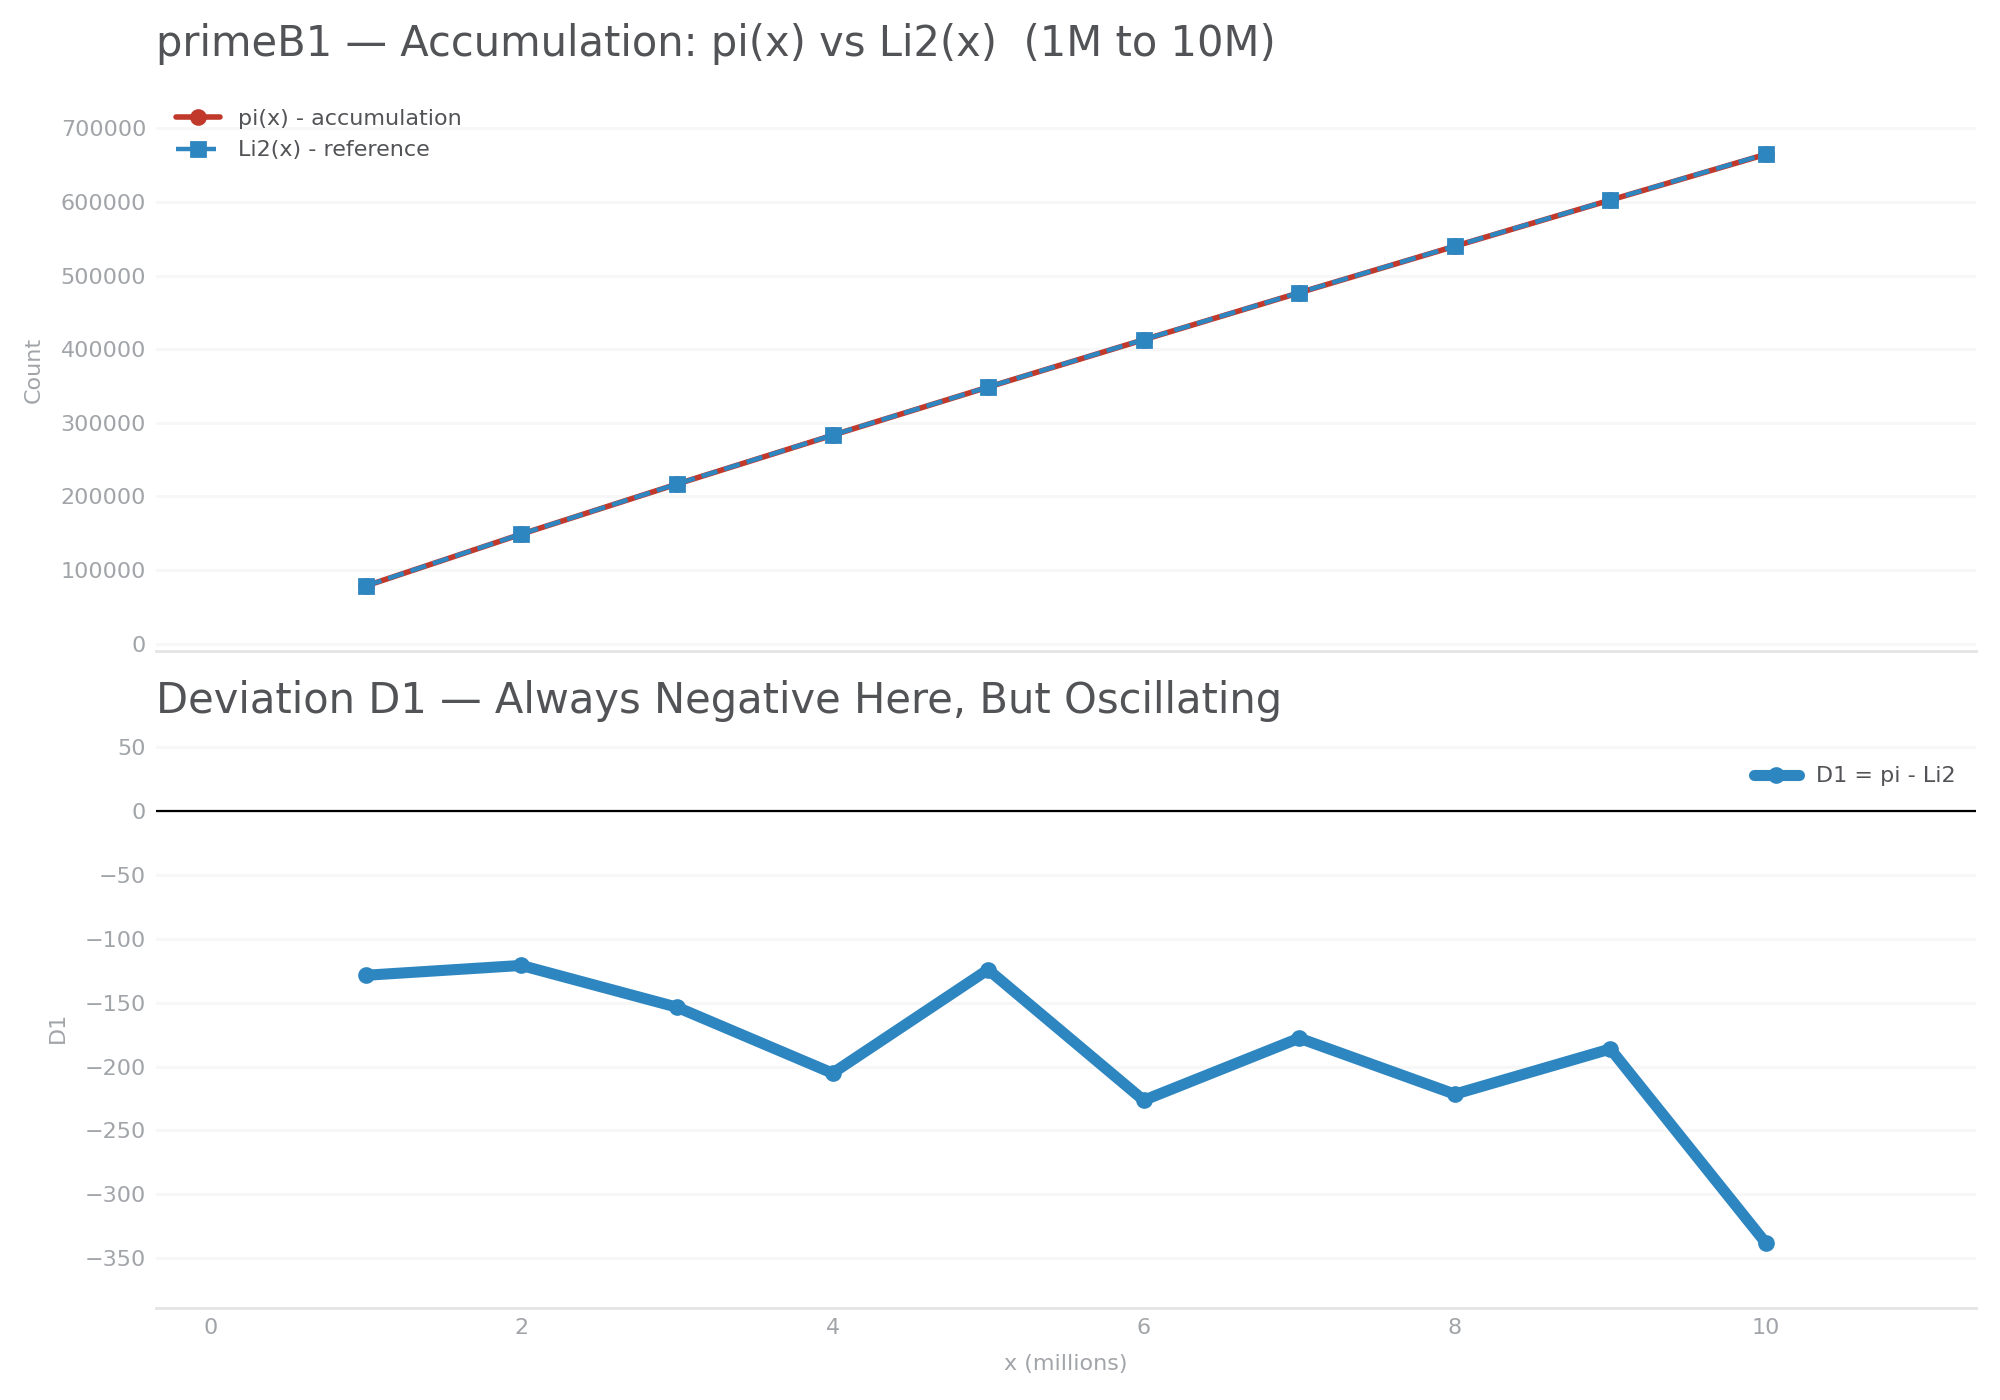
\includegraphics[width=0.32\textwidth]{primeB1.png}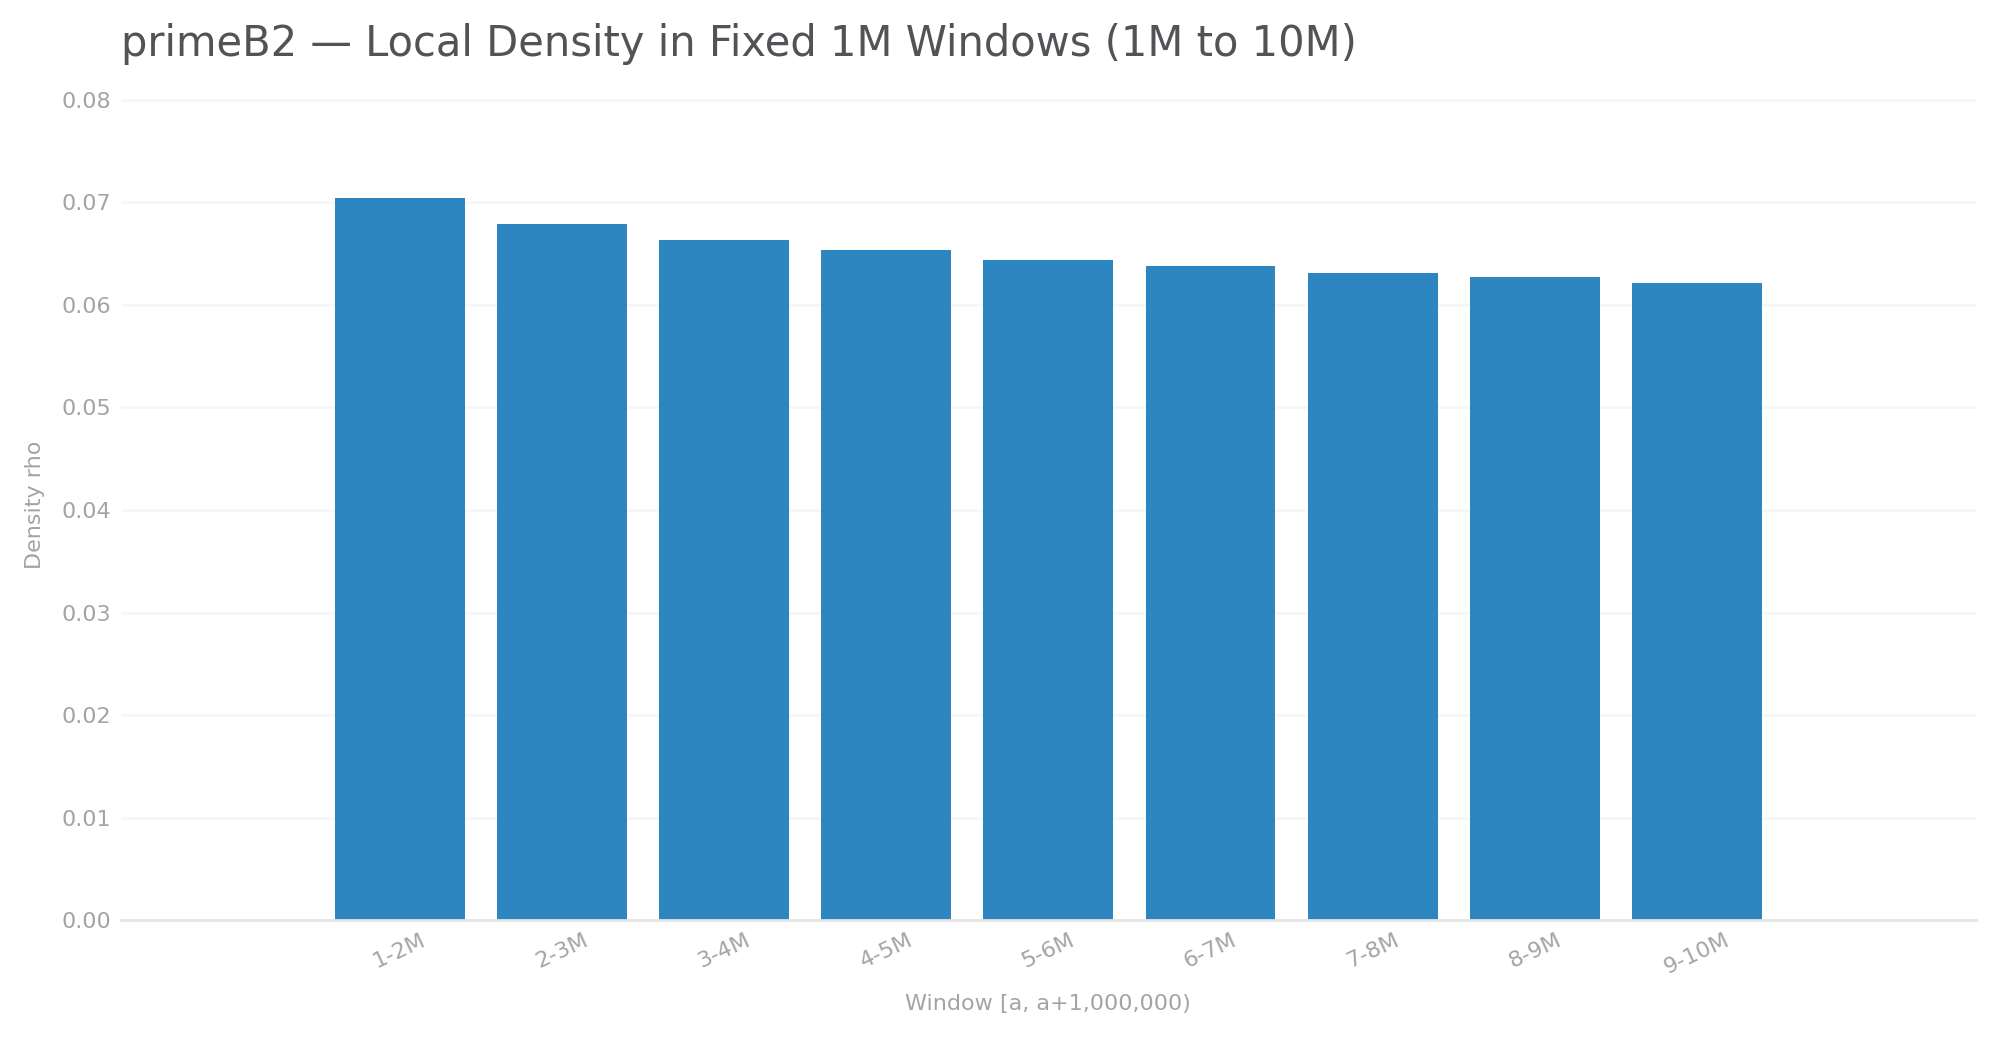
\includegraphics[width=0.32\textwidth]{primeB2.png}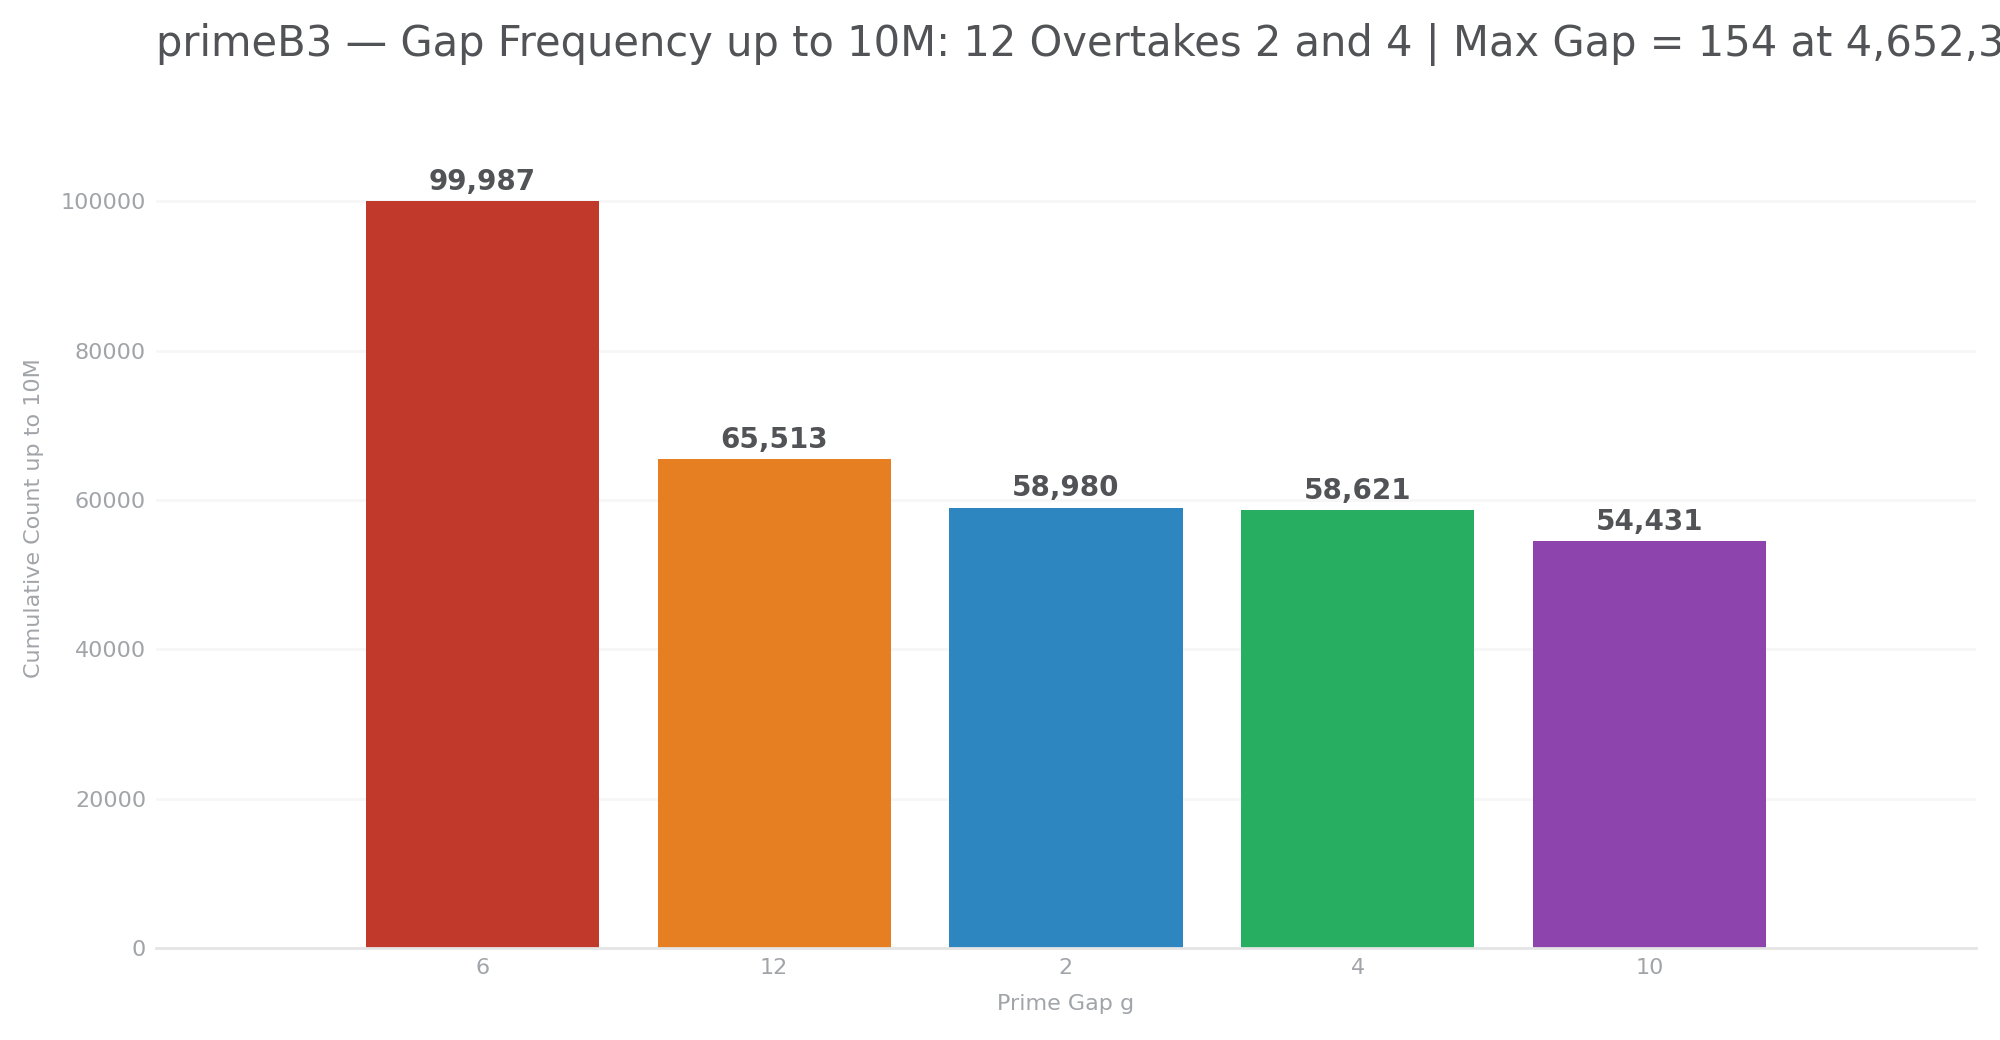
\includegraphics[width=0.32\textwidth]{primeB3.png}\caption{Stage $B$: Deviation $D_1$, Density $\rho_k$, and Gap Frequencies}\end{figure}
\begin{figure}[H]\centering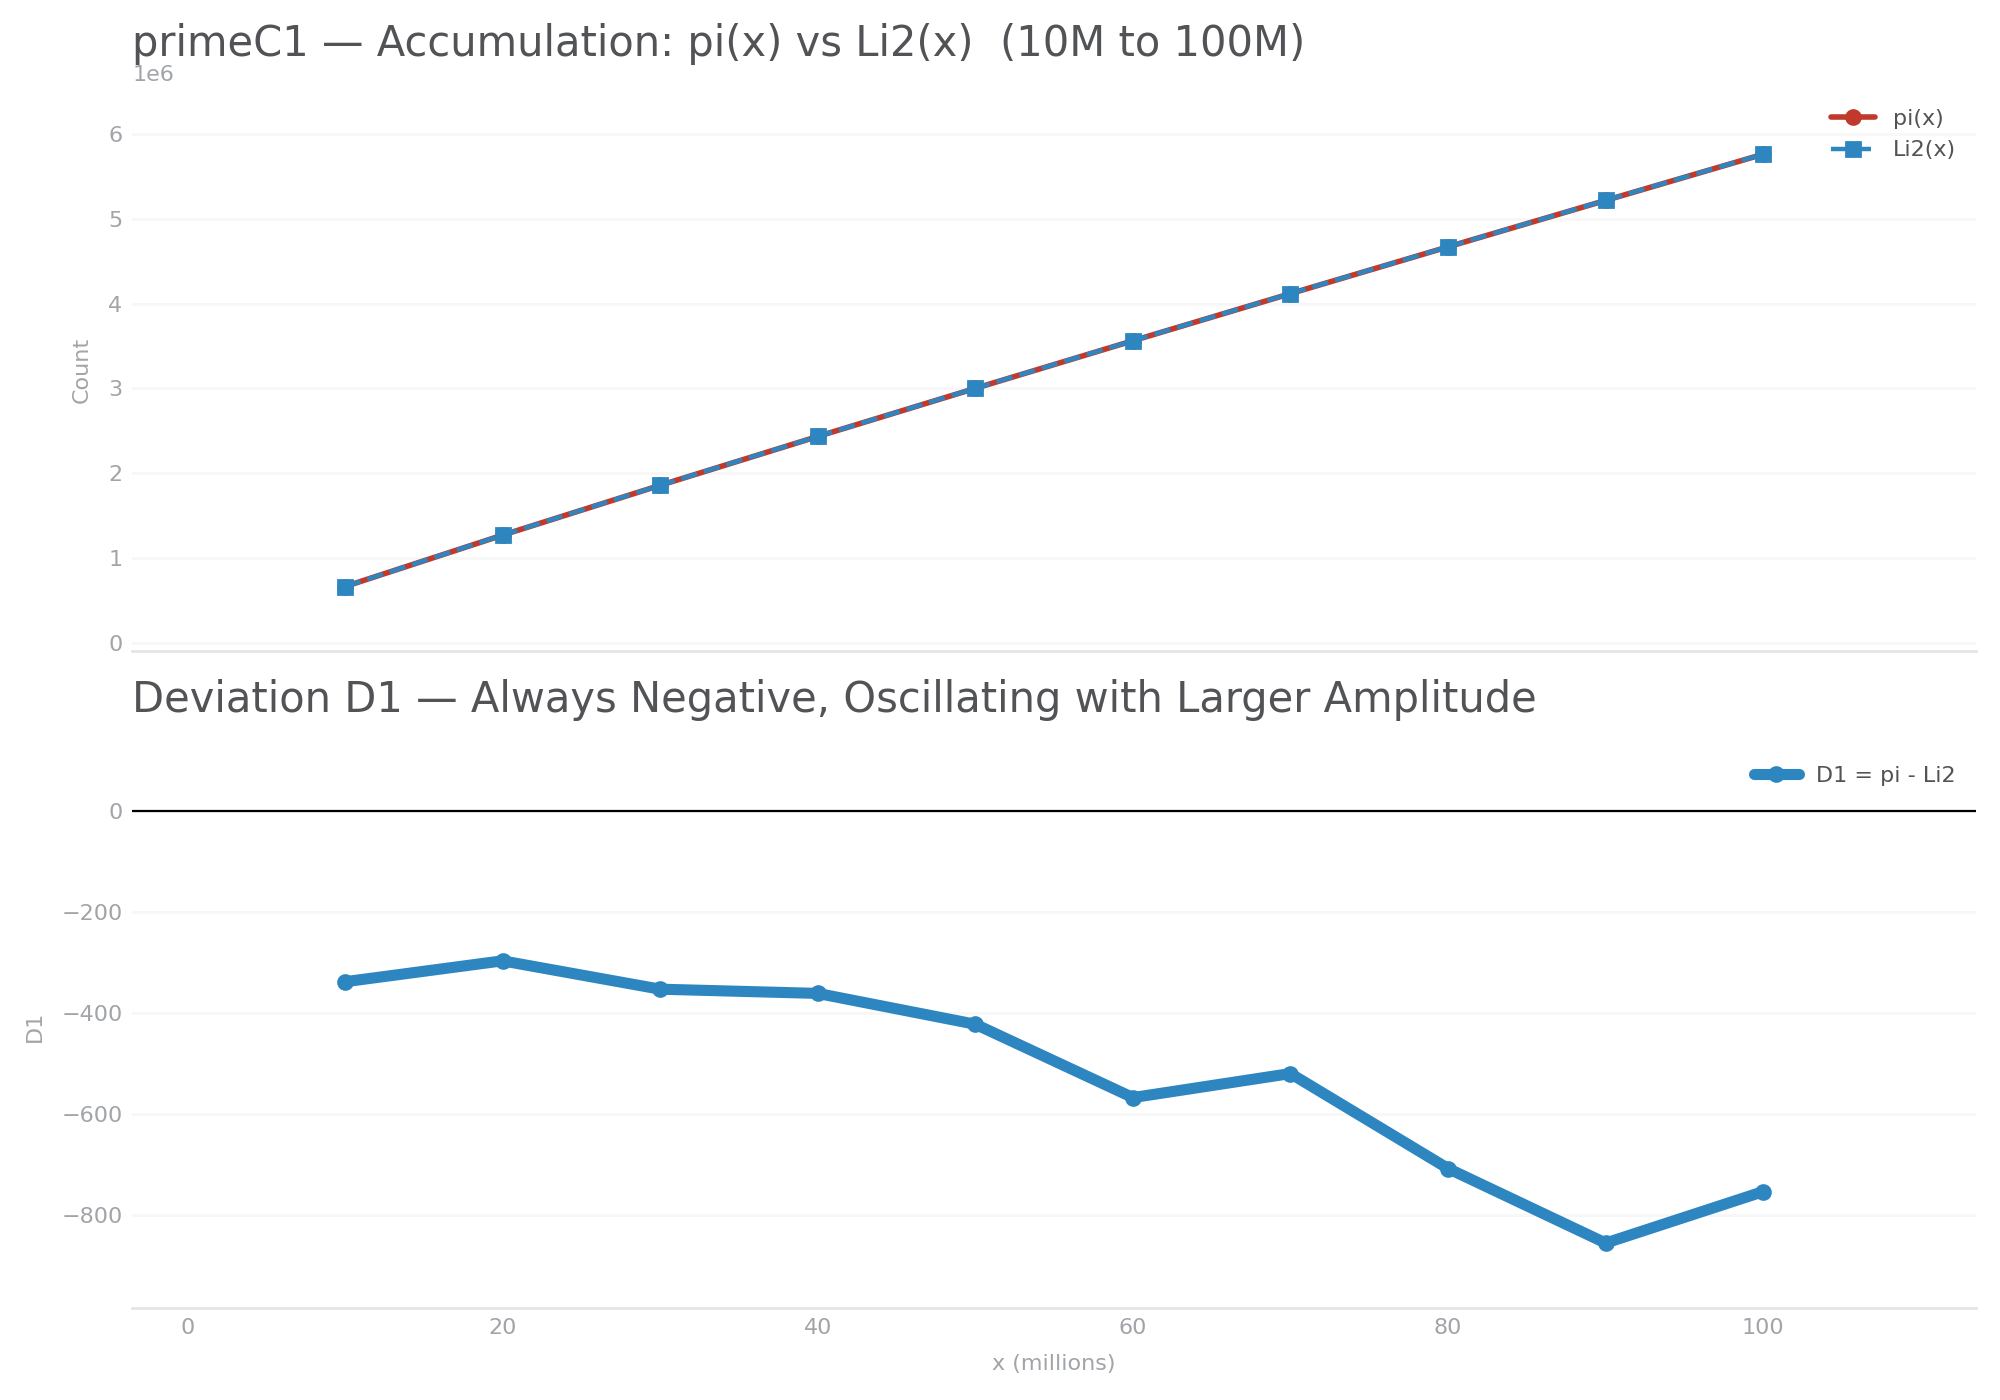
\includegraphics[width=0.32\textwidth]{primeC1.png}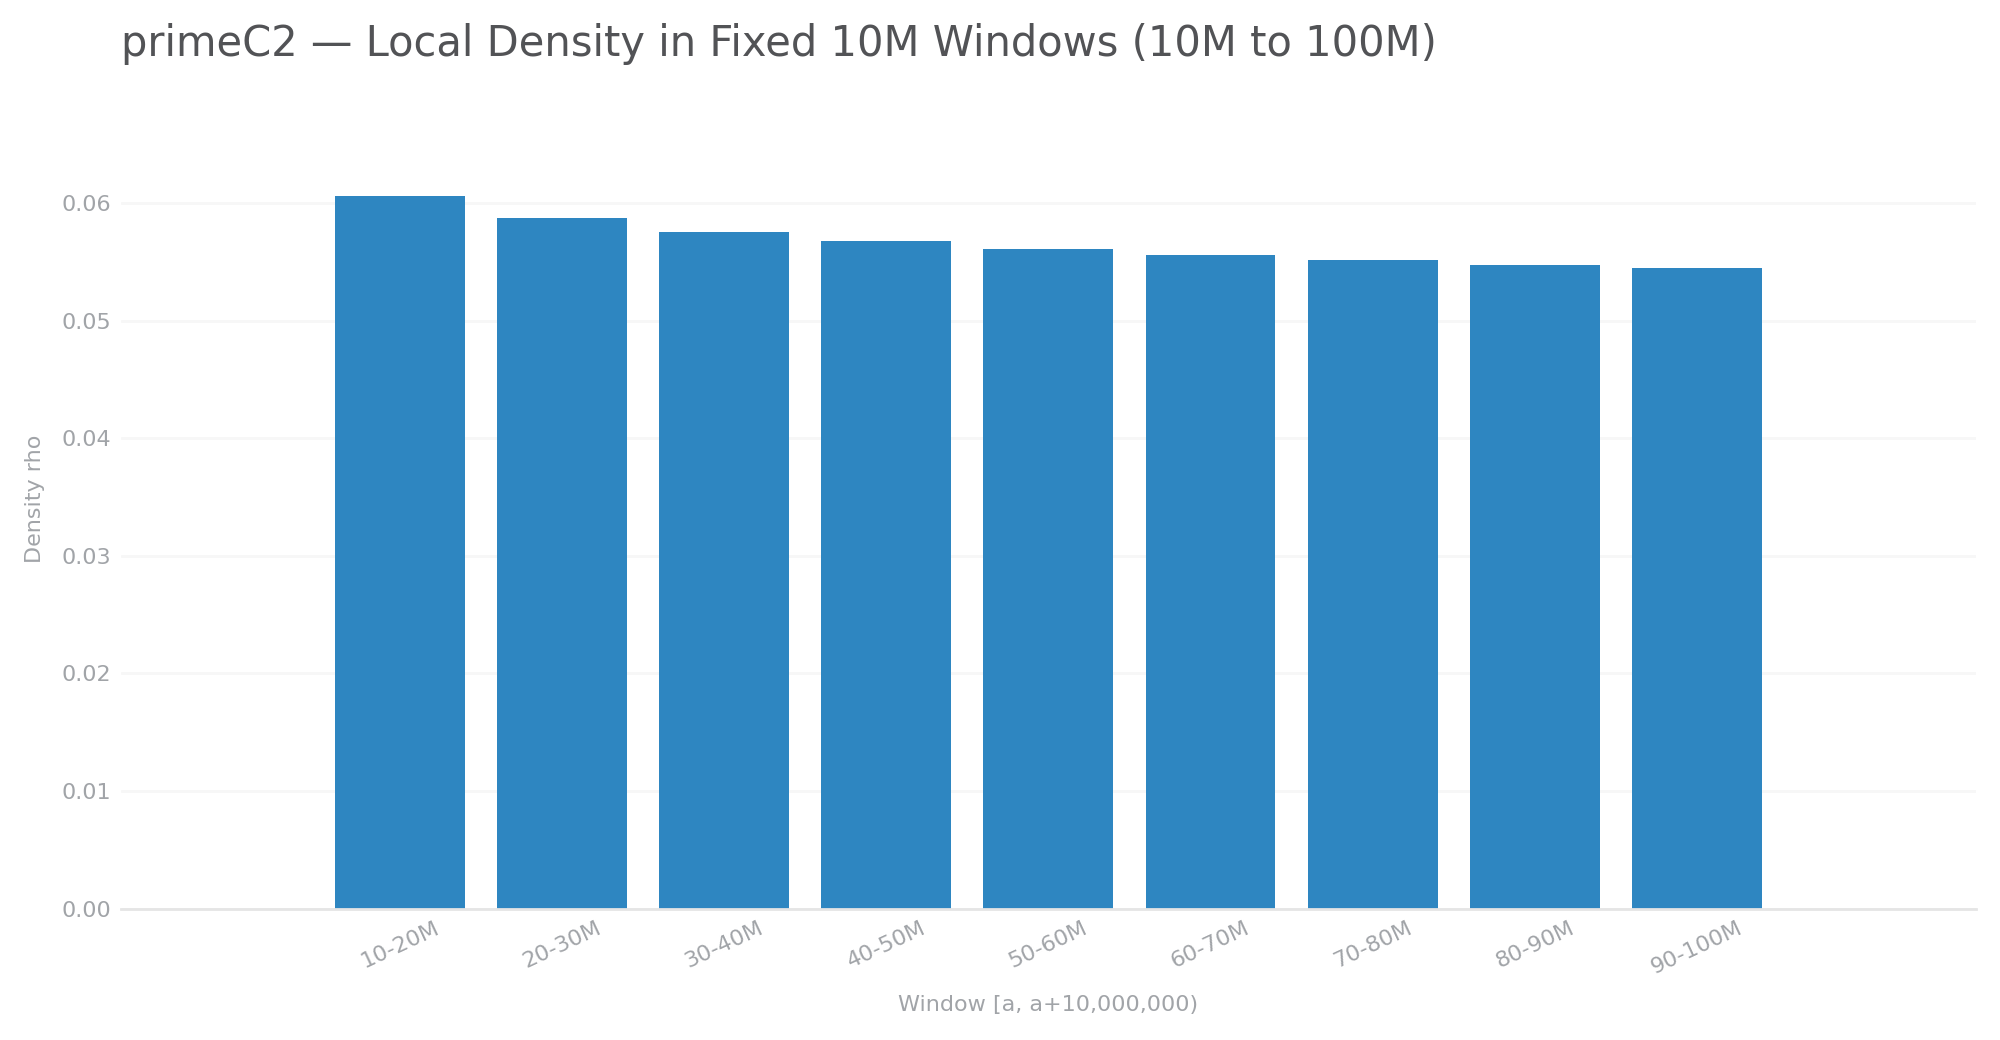
\includegraphics[width=0.32\textwidth]{primeC2.png}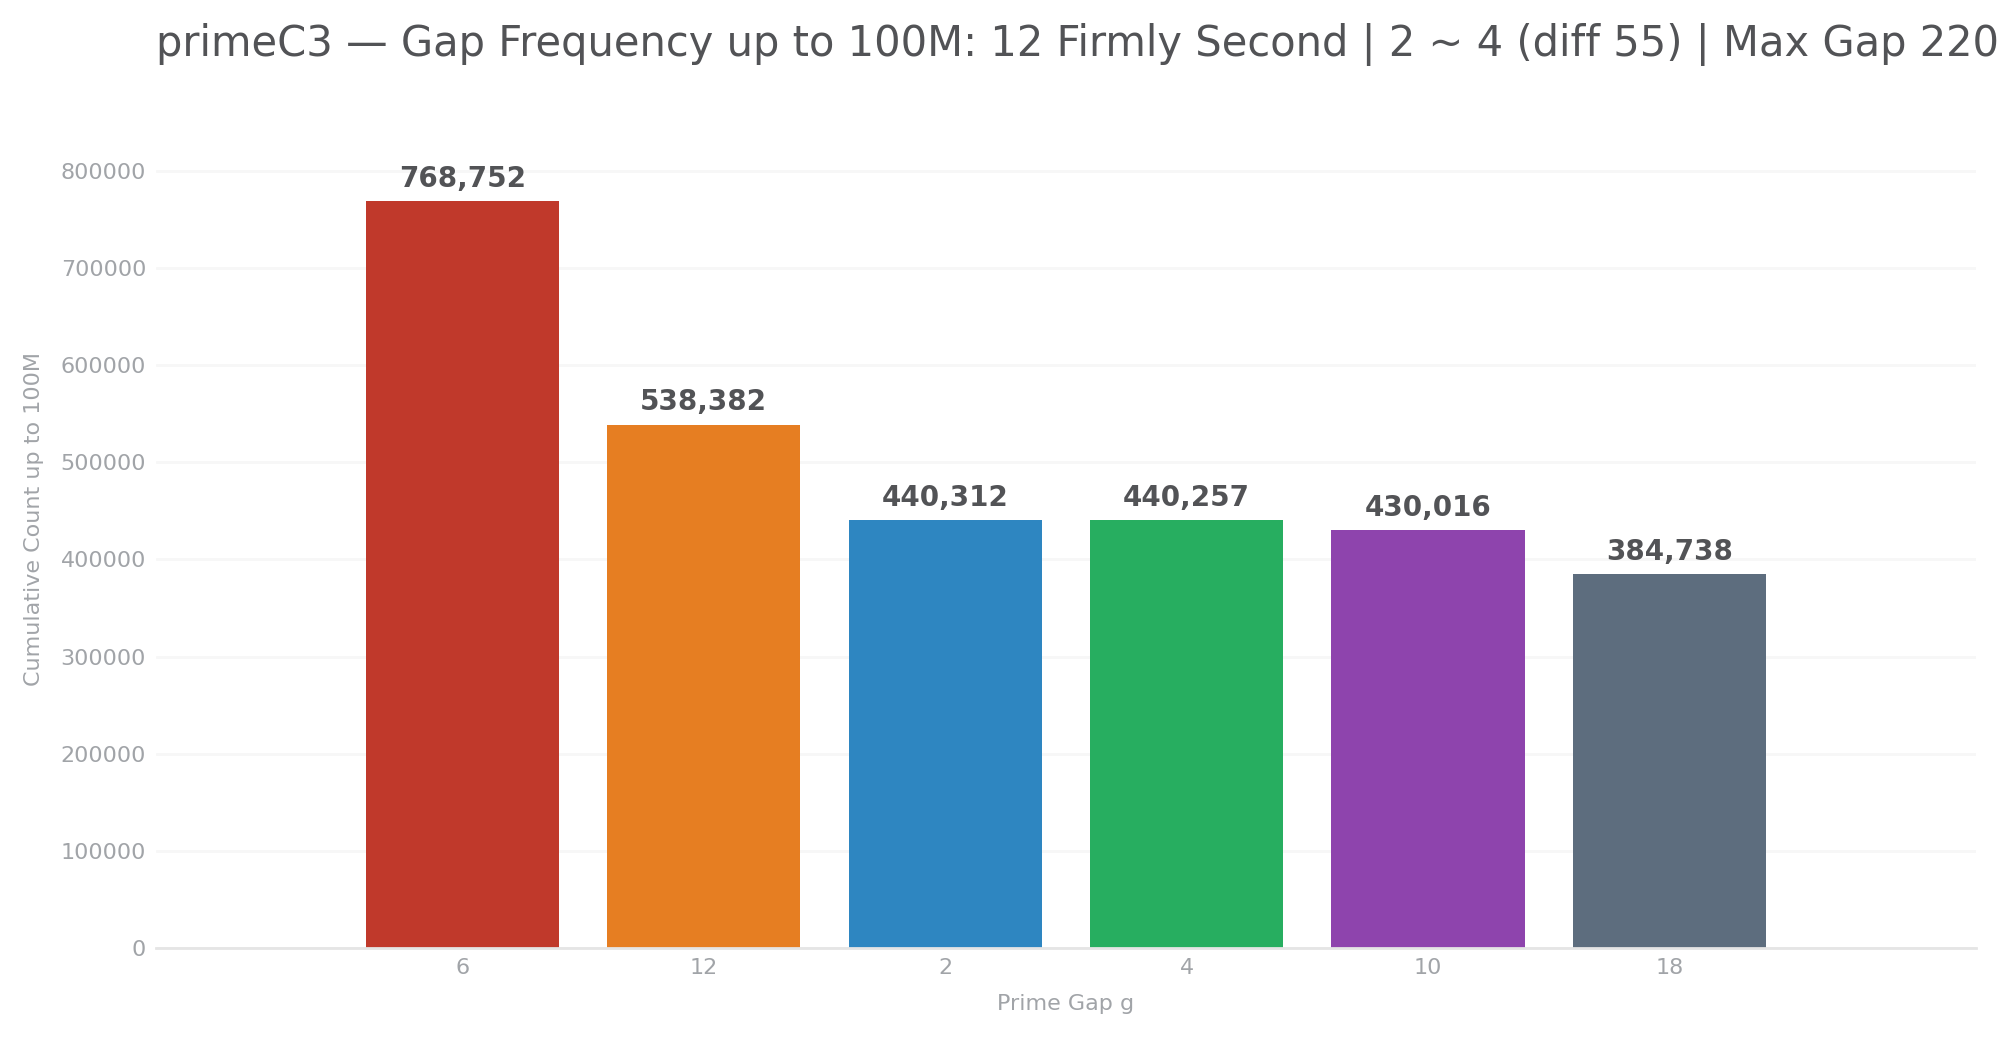
\includegraphics[width=0.32\textwidth]{primeC3.png}\caption{Stage $C$: Deviation $D_1$, Density $\rho_k$, and Gap Frequencies}\end{figure}
\begin{figure}[H]\centering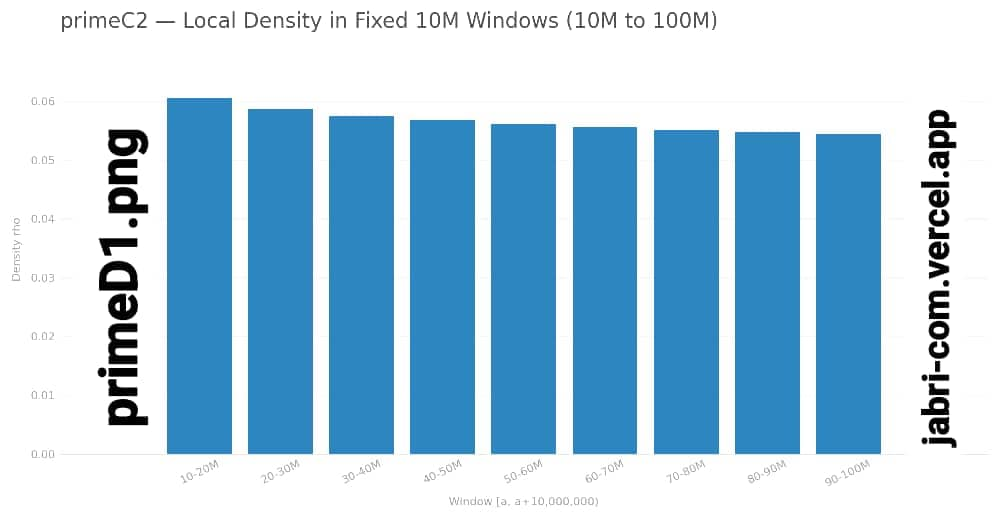
\includegraphics[width=0.32\textwidth]{primeD1.png}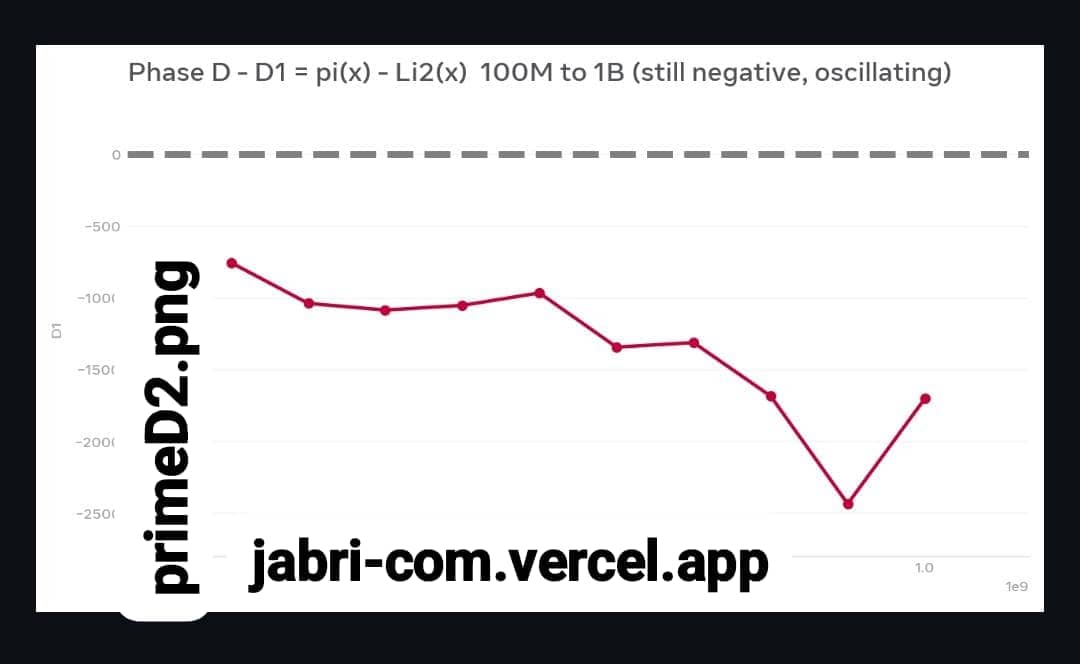
\includegraphics[width=0.32\textwidth]{primeD2.png}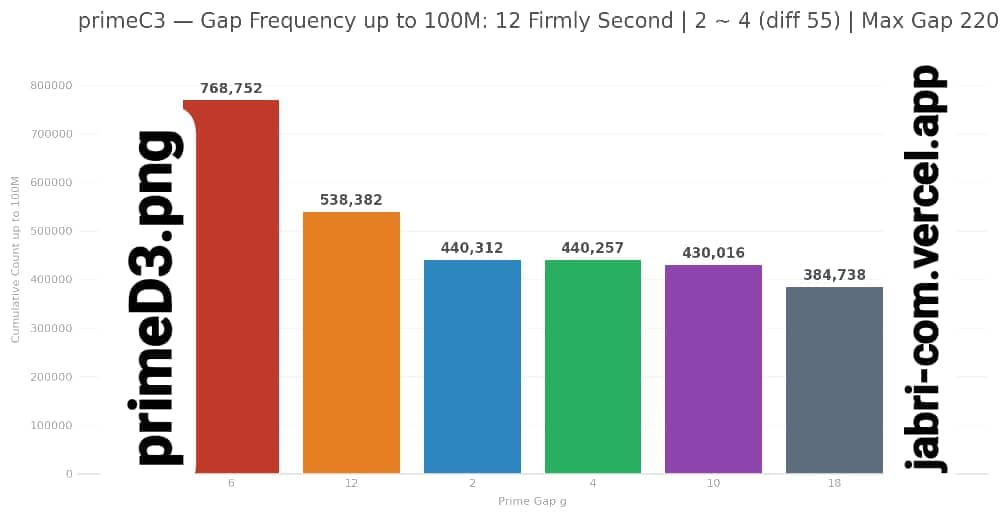
\includegraphics[width=0.32\textwidth]{primeD3.png}\caption{Stage $D$: Deviation $D_1$, Density $\rho_k$, and Gap Frequency Shift}\end{figure}
% ==========================================
\section{Cross-Stage Synthesis: Adjacency Structure and Primorial Sieve}
\subsection{Central Question}
Can the negative lag-1 autocorrelation of adjacent prime gaps ($r_1 < 0$) be related to small-prime divisibility constraints, without assuming gap independence or a prior asymptotic law? This section is limited to the first $1,000,000$ primes ($p_{10^6} = 15,485,863$). No $N = 10,000,000$ computation is claimed, and no Hurst / DFA estimate is reported as proven.
\subsection{Adjacency Measures}
\[
r_k = \frac{\sum_{i=1}^{n-k} (g_i - \bar{g})(g_{i+k} - \bar{g})}{\sum_{i=1}^{n} (g_i - \bar{g})^2}
\qquad
R_{\text{stat}} = \frac{1}{n-1} \sum_{i=1}^{n-1} \frac{\min(g_i, g_{i+1})}{\max(g_i, g_{i+1})}
\]
A shuffled control can be used to evaluate whether the observed lag-1 correlation is distinguishable from correlations generated by random reorderings that preserve the marginal gap distribution. The outcome of this control is not assumed in advance.
\subsection{Primorial Sieve Model}
For $M = \prod_{p \le p_k} p$, e.g. $M = 6, 30, 210, 2310, 30030, 510510$, the exact cycle of residues coprime to $M$ gives a closed gap cycle. For $M = 30$ ($\phi(30) = 8$):
\[
\mathcal{C}_{30} = [6, 4, 2, 4, 2, 4, 6, 2]
\]
These purely arithmetic cycles already have $r_{\text{sieve}} < 0$. These cycles show that adjacent-gap dependence can arise from modular constraints alone in a finite arithmetic model. This does not establish that the same mechanism causes the measured correlation in the actual prime sequence, and it does not prove a general asymptotic law.
% ==========================================
\section{Extra-Memory Test of the Exact Gap Value (M1-E)}
The question is not only whether the current gap class is associated with the next gap class, but whether the exact numerical value of the current gap carries additional information beyond its size class alone.
Let the consecutive gap sequence be $(g_1,g_2,\ldots,g_m)$, and let \(S_n\in\{1,2,3\}\) be the class of gap \(g_n\):
\[
\text{Small}: g\leq6, \quad \text{Medium}: 8\leq g\leq14, \quad \text{Large}: g\geq16.
\]
Model M1 tests $P(S_{n+1}\mid S_n)$, while M1-E tests $P(S_{n+1}\mid g_n)$. Hence the central question is: Does $g_n$ add predictive information beyond $S_n$ when predicting $S_{n+1}$?
\paragraph{Test protocol (frozen, in progress).}
\begin{enumerate}
    \item Splitting transition data into training and test sets at \(50\%/50\%\).
    \item Representing exact gap values up to \(30\), and using fixed logarithmic bins for larger gaps.
    \item A merging threshold of \(200\), a fixed ascending merging system, with Laplace smoothing \(\alpha=1\). Merging detail: rare categories are merged ascendingly from largest to smallest until each merged category reaches at least $200$ in training; ties in frequency are broken by choosing the smaller value first, under the seed below. This is a test setting, not a statistical guarantee.
    \item Block Bootstrap with block length \(100\) (fixed test setting), and \(B=2000\) repetitions.
    \item Evaluating improvement with Log-Loss, with the Pearson coefficient evaluated independently and the two judgments not merged into a single criterion.
    \item No change to the protocol after inspecting results.
\end{enumerate}
\paragraph{Implementation definitions (frozen).}
\begin{enumerate}
    \item \textbf{Split:} Chronological sequential split. The first half of the ordered transition sequence is training and the second half is test. Transitions are not randomly shuffled across the split.
    \item \textbf{Pearson, defined:} The Pearson coefficient reported independently is the lag-1 correlation $r_1$ between consecutive class codes $S_n$ and $S_{n+1}$, with encoding Small $=1$, Medium $=2$, Large $=3$. This encoding imposes a numerical order on the classes, so $r_1$ is interpreted as a linear rank correlation on this encoding specifically, not as a general measure of all forms of dependence.
    \item \textbf{Bootstrap, paired:} Block Bootstrap resamples blocks of length $100$ from test transitions. The same resampled blocks are used for both M1 and M1-E in each repetition, so the comparison is paired. The confidence interval for $\Delta = \text{Log-Loss}_{M1} - \text{Log-Loss}_{M1-E}$ is obtained from percentiles of the $B=2000$ paired values.
    \item \textbf{Seed, scoped:} \texttt{SEED = 20261120} is a fixed reproducibility setting for the stochastic part (Bootstrap resampling and tie-breaking). The chronological split is deterministic and is not decided by the seed. The seed alone does not prove correctness.
\end{enumerate}
\paragraph{Evaluation criterion.}
M1-E performance is measured on test data compared with M1. A lower Log-Loss is interpreted as an improvement in predictive performance, with magnitude and uncertainty evaluated under the adopted protocol. Absence of a clear improvement means no additional predictive evidence was found within the tested data and settings; it does not prove absence of additional information in general.
\paragraph{Test status.}
The M1-E protocol is specified and frozen, but its execution and final result on the actual prime-gap data are still in progress. Therefore no simulation result is presented as a result computed from the original prime sequence, and no result is stated in advance.
\subsection{Class-Order Test and Shuffled Control}
On the ordered class sequence, with the encoding above:
\[
r_1=-0.03006.
\]
This indicates a weak negative linear correlation between current and next gap class. To distinguish order effect from marginal distribution effect, a Shuffled Control can be performed, reordering the sequence while preserving class frequencies. The negative correlation alone is not interpreted as proof of a specific causal mechanism, nor is absence of strong linear correlation evidence for absence of all dependence.
% ==========================================
\section{Discussion, Methodological Verification, and Limitations}
\subsection{What Changed vs. What Remained Invariant}
\begin{itemize}
\item \textbf{At checkpoints:} $D_1 < 0$ and $D_2 > 0$ held at every documented closure point from $A$ to $D$; gaps $6$ and $12$ retained Ranks $1$ and $2$ across all stages.
\item \textbf{Rank Difference in Stage $D$:} Up to Stage $C$, the cumulative top six gaps were ordered $(6, 12, 2, 4, 10, 18)$. Inside Stage $D$ alone, the ranking was $(6, 12, 10, 4, 2, 18)$, with gap $10$ at Rank $3$ and gaps $4$ and $2$ differing by only $228$ occurrences ($2{,}984{,}422$ vs. $2{,}984{,}194$). A difference across ranges is recorded as a comparison observation; it does not by itself establish a dynamic pattern or mechanism.
\item \textbf{Primorial Modular Constraint:} Finite primorial residue cycles provide an arithmetic example in which adjacent-gap dependence can arise from modular constraints alone. This motivates investigation of adjacency structure, but does not establish that the measured correlation in the actual prime sequence is caused solely by these constraints. The measured value in M1 is $r_1 = -0.03006$, a weak linear correlation, not proof of repulsion or of a causal mechanism.
\end{itemize}
\subsection{Isolation of Verification Sieve Artifacts}
During independent verification of Stage $D$, a defective verification script that erroneously included $1$ as a prime nearly introduced an unwarranted adjustment. Isolating and discarding that artifact — strictly enforcing $1 \notin \mathbb{P}$ — was integral to validating the exact Stage $D$ gap count ($45{,}086{,}079$).
\subsection{Explicit Scope Boundaries}
Stages $A$--$D$ do not by themselves establish that $D_1(x)$ remains negative beyond $10^9$, nor any periodic law from $\Delta D_1$ fluctuations ($-750.4$ to $+732.688$), nor whether the near-tie between gaps $2$ and $4$ persists or reverses in Stage $E$ ($1\text{B} \rightarrow 10\text{B}$).
\subsection{Empirical Observation}
\begin{quote}
\textbf{Empirical observation:} Within the computational range up to $10^9$, the compared ranges showed a difference in the ranking of prime-gap frequencies $g_n$. This difference coincided with decreasing prime density across the studied numerical windows. This observation is recorded as an empirical comparison between frequency behaviour and density, without assuming a causal or deterministic periodic relation.
\end{quote}
% ==========================================
\section{Committee Questions}
\textbf{Why exclude 1?} Because $1$ is not prime; including it creates a false gap.

\textbf{Why is gap 1 the only odd gap?} After $2$, all primes are odd, and the difference of two odds is even.

\textbf{Can you predict the next gap?} Not from $r_1$ alone; it is a weak linear correlation on the documented encoding, and is insufficient for prediction.

\textbf{Is this a general law?} This is what was observed in the measured range. Evaluation of its naming and significance is left to the reader and referees.

\subsection*{Extra-Memory Test Protocol (M1-E) --- Summary for the Committee}
M1-E tests whether the exact value $g_n$ adds predictive information beyond class $S_n$ when predicting $S_{n+1}$, comparing $P(S_{n+1}\mid S_n)$ with $P(S_{n+1}\mid g_n)$. The protocol is frozen and in progress (chronological 50\%/50\% split, exact representation up to $30$, merging threshold $200$, Laplace smoothing $\alpha=1$, paired Block Bootstrap with block length $100$ and $B=2000$, evaluation by Log-Loss, $r_1$ evaluated independently). The final result has not yet been adopted, and no simulation is presented as a result from the original sequence.
\textbf{How does M1-E differ from the shuffled control?} The shuffled control is only an auxiliary test of order effect; it preserves class distribution and breaks order. Alone, it does not prove an exclusive cause, and does not substitute for the exact-value test.
\textbf{Why seed \texttt{SEED = 20261120}?} For reproducibility and to prevent biased selection of results; derived from the protocol freeze date (20 November 2026). It governs only the stochastic part; the chronological split is deterministic.
\textbf{Did $r_1=-0.03006$ prove repulsion or absence of memory?} No. It is a weak negative linear correlation on the documented encoding, conditional on correctness of calculation. Pearson does not measure all forms of dependence, does not prove a specific causal mechanism, and does not rule out memory in general. M1-E was designed to test whether the exact value adds information that classes did not reveal.
% ==========================================
\section{Reproducibility and Conclusion}
All prime-generation and counting computations reported in Stages $A$--$D$ were performed in \texttt{Python 3} using the Sieve of Eratosthenes, with $1$ excluded from the prime set. The M1-E protocol and its reproducibility settings have been frozen, but the final M1-E evaluation on the actual prime-gap dataset remains in progress. The code is deposited when the final Prime version is ready for deposit, after three closures: (1) fixing the counting script and data production, (2) completing the M1 and M1-E tests or stating precisely what was and was not executed, (3) matching the tables and numbers in the paper with the files produced by the final run. The code is then uploaded to a GitHub repository, a specific version (Release/Tag) is fixed, and the link to that version — not a mutable link to the latest GitHub files — is placed on the first DOI/Zenodo page.

This study presents the results of the computational survey of prime gaps within the specified range, and what comparisons showed in terms of changes in prime density, gap distribution, and frequency rankings. These results form a basis for later comparisons and tests, including the test of additional information that the exact gap value may carry. Evaluation of the results, their implications, and the place of this work is left to the reader and referees.

\textbf{Later work:}
\begin{itemize}
\item Extending the segmented sieve to $N = 10^{11}$.
\item Building Markov transition matrices for the three gap classes to quantify mutual information between $g_n$ and $g_{n+1}$.
\end{itemize}
\begin{thebibliography}{9}
\bibitem{hardy} G. H. Hardy and E. M. Wright, \textit{An Introduction to the Theory of Numbers}, 6th ed., Oxford University Press, 2008.
\bibitem{lemke} R. J. Lemke Oliver and K. Soundararajan, ``Unexpected biases in the distribution of consecutive primes,'' \textit{PNAS}, vol. 113, no. 31, pp. E4446--E4454, 2016.
\bibitem{granville} A. Granville, ``Harald Cram\'er and the distribution of prime numbers,'' \textit{Scandinavian Actuarial Journal}, vol. 1995, no. 1, pp. 12--28, 1995.
\end{thebibliography}
\end{document}
